\chapter{Requisitos do sistema}
\addcontentsline{toc}{chapter}{Requisitos do sistema}

\section{Requisitos funcionais}

Os requisitos funcionais do sistema são definidos pelas características para que um MVP possa ser entregue.
Os requisitos são descritos no diagrama de caso de uso abaixo.

\begin{figure}[!htb]
    \label{figure_diagrama_caso_uso}
    \centering
    \caption{Diagrama de caso de uso} \label{includegraphics_diagrama_caso_uso}
    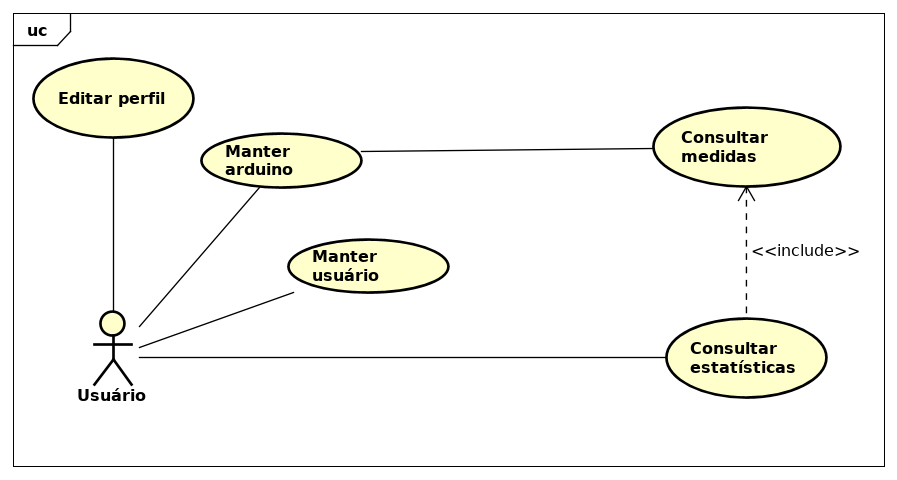
\includegraphics[scale=0.6]{diagrams/caso_de_uso.png}
    \hfill
\end{figure}

Os atores do sistema foram definidos com o o próprio sistema, que poderá realizar acesso a alguns casos de uso e o usuário final.
Seguem abaixo as especificações dos casos de uso.

\begin{table}
    \ABNTEXfontereduzida
    \caption{Especificações do caso de uso capturar dados meteorológicos}
    \label{my-label}
    \begin{tabular}{{l}|p{9.0cm}}

    \hline

    \multicolumn{2}{c}{\textbf{Capturar dados meteorológicos}} \\

    \hline
    Descrição & Captura os dados meteorológicos através de sensores conectados ao microcontrolador arduino e os envia através de requisição HTTP para a API \\

    \hline

    Atores & Sistema \\

    \hline

    \multirow{2}{*}{Pré-condições} & Credenciais de acesso a API \\
    & API em correto funcionamento \\

    \hline

    \multirow{2}{*}{Exceções e fluxos alternativos} & Em caso de perca de conexão com internet ou a API, armazena as informações temporariamente no Arduino \\

    \hline

    \end{tabular}
\end{table}

\begin{table}
    \ABNTEXfontereduzida
    \caption{Especificações do caso de uso armazenar dados meteorológicos}
    \label{my-label}
    \begin{tabular}{{l}|p{9.0cm}}

    \hline

    \multicolumn{2}{c}{\textbf{Armazenar dados meteorológicos}} \\

    \hline
    Descrição & Após receber os dados captados pelo arduino, a api os valida e então, os armazena em banco de dados \\

    \hline

    Atores & Sistema \\

    \hline

    \multirow{2}{*}{Pré-condições} & Banco de dados em correto funcionamento  \\
    & Recebimento de dados através das rotas da API \\

    \hline

    \multirow{2}{*}{Exceções e fluxos alternativos} & Em caso de dados inválidos, a API os descarta \\

    & Em caso de perca de conexão com banco de dados, a API os armazena em memória \\

    \hline

    \end{tabular}
\end{table}

\begin{table}
    \ABNTEXfontereduzida
    \caption{Especificações do caso de uso realizar consultas com filtros}
    \label{my-label}
    \begin{tabular}{{l}|p{9.0cm}}

    \hline

    \multicolumn{2}{c}{\textbf{Realizar consultas com filtros}} \\

    \hline
    Descrição & Recebe do usuário os filtros para seleção das informações, então, realiza uma análise estatística dos dados requeridos e os exibe para o usuário utilizando gráficos. \\

    \hline

    Atores & Usuário \\

    \hline

    \multirow{3}{*}{Pré-condições} & Credenciais de acesso ao banco de dados para realizar as consultas  \\
    & Banco de dados em correto funcionamento \\
    & Filtros corretos passados pelo usuário \\

    \hline

    \multirow{2}{*}{Exceções e fluxos alternativos} & Caso ele não encontre dados na seleção, exibe uma mensagem de não encontrado  \\

    & Em caso de perca de conexão com banco de dados, exibe uma tela de erro ao usuário \\

    \hline

    \end{tabular}
\end{table}

\begin{table}
    \ABNTEXfontereduzida
    \caption{Especificações do caso de uso realizar análise estatística dos dados}
    \label{my-label}
    \begin{tabular}{{l}|p{9.0cm}}

    \hline

    \multicolumn{2}{c}{\textbf{Realizar análise estatística dos dados}} \\

    \hline
    Descrição & Realiza calculo estatístico de informações, retornando informações relevantes como média, moda e desvio padrão. \\

    \hline

    Atores & Usuário \\

    \hline

    \multirow{2}{*}{Pré-condições} & Credenciais de acesso ao banco de dados  \\
    & Banco de dados em correto funcionamento \\

    \hline

    \multirow{2}{*}{Exceções e fluxos alternativos} & Caso não existam dados para serem analisados, joga uma exceção de argumentos inválidos  \\

    \end{tabular}
\end{table}

\section{Requisitos não funcionais}

Os requisitos não funcionais do sistema complementam os requisitos funcionais, como melhorias para as especificações.

\subsection{Segurança}

O projeto precisa trabalhar de forma segura, então, esse requisito pede para que a API possua autenticação das aplicações clientes e que também, a aplicação web possua autenticação, para o usuário visualizar as informações e realizar consultas, ele precisa estar autenticado.

\subsection{Disponibilidade}

Para garantir uma melhor análise e fidelidade dos dados, o sistema precisa funcionar durante 24 horas por dia e 7 dias por semana, para isso, redundâncias precisam ser trabalhadas.

\subsection{Performance}

Outro requisito não funcional do sistema é a performance, as informações precisam ser processadas de forma rápida, problemas como lentidão no processamento podem acabar acavalando a aplicação.
